%!TEX program = lualatex
% SPDX-License-Identifier: CC-BY-SA-4.0
\documentclass[11pt]{article}

\usepackage{iftex}
\ifLuaTeX\else
  \PackageError{vintage-latex}{This example requires LuaLaTeX}
    {Run lualatex, not pdflatex or xelatex.}
\fi

\usepackage{fontspec}
\usepackage{xcolor}
\usepackage{geometry}
\usepackage[tracking=true,protrusion=false,expansion=false]{microtype}
\usepackage{tikz}
\usetikzlibrary{lindenmayersystems,shapes.geometric,patterns.meta}

\defaultfontfeatures{Renderer=HarfBuzz}
\setmainfont{EB Garamond}[Numbers={OldStyle,Proportional}]
\definecolor{platepaper}{HTML}{F3E9D7}
\definecolor{printerink}{HTML}{25201B}
\pagecolor{platepaper}
\color{printerink}
\geometry{a4paper,top=22mm,bottom=22mm,left=26mm,right=26mm}
\pagestyle{empty}

% Two branching grammars. Each grows one arm; six rotated copies make the
% hexagonal crystal. Angles of 60 degrees keep every branch on the lattice.
\pgfdeclarelindenmayersystem{stellar}{
  \rule{F -> F[+F][-F]F}
}
\pgfdeclarelindenmayersystem{fernlike}{
  \rule{F -> FF[+F[-F]][-F[+F]]F}
}

\tikzset{
  fieldedge/.style={draw=printerink,line width=.75pt},
  crystal/.style={draw=printerink,line width=.42pt,line cap=round,
                  line join=round},
  fine crystal/.style={crystal,line width=.3pt},
  vignette/.style={pattern={Lines[angle=45,distance=1.7pt,line width=.18pt]},
                   pattern color=printerink!55}
}

% A circular microscope field: hatched surround, clipped drawing, then the
% edge, a fiducial cross, and the graduated stage micrometer below.
\newcommand{\fieldofview}[3]{% #1 radius in cm, #2 label, #3 drawing code
  \begin{tikzpicture}[x=1cm,y=1cm]
    \path[vignette] (-#1-.55,-#1-.55) rectangle (#1+.55,#1+.55);
    \fill[platepaper] (0,0) circle[radius=#1];
    \begin{scope}
      \clip (0,0) circle[radius=#1];
      #3
    \end{scope}
    \draw[fieldedge] (0,0) circle[radius=#1];
    \draw[printerink,line width=.25pt]
      (-#1,0)--(-#1+.22,0) (#1,0)--(#1-.22,0)
      (0,-#1)--(0,-#1+.22) (0,#1)--(0,#1-.22);
    \draw[printerink,line width=.25pt]
      (-#1-.55,-#1-.55) rectangle (#1+.55,#1+.55);
    \node[below,font=\small\itshape,inner sep=6pt] at (0,-#1-.55) {#2};
  \end{tikzpicture}%
}

\begin{document}

\begin{center}
  {\small\textls[120]{\textsc{Tab.\ VII}}}\par
  \vspace{.3em}
  {\Large Figures of Snow Crystals}\par
  \vspace{.2em}
  {\itshape observed under the microscope during the frost of January}
\end{center}

\vspace{1.4em}

\begin{center}
\fieldofview{2.5}{Fig.\ 1.\ Simple hexagonal plate.}{
  \foreach \s in {2.05,1.55,1.05,.55} {
    \node[regular polygon,regular polygon sides=6,minimum size=\s cm,
          fine crystal,inner sep=0pt] at (0,0) {};
  }
  \foreach \a in {0,60,...,300} {
    \draw[fine crystal] (0,0) -- (\a:2.05);
  }
  \node[regular polygon,regular polygon sides=6,minimum size=2.05cm,
        crystal,inner sep=0pt] at (0,0) {};
}
\hspace{1.5em}
\fieldofview{2.5}{Fig.\ 2.\ Stellar dendrite.}{
  % Order 2 keeps the side branches short of one another; at order 3 the
  % branches of neighbouring arms meet and the figure closes into a lattice.
  \foreach \a in {0,60,...,300} {
    \draw[crystal,rotate=\a]
      l-system[l-system={stellar,axiom=F,order=2,step=.5cm,angle=60}];
  }
  \node[regular polygon,regular polygon sides=6,minimum size=.62cm,
        crystal,inner sep=0pt] at (0,0) {};
}
\end{center}

\vspace{1.4em}

\begin{center}
\fieldofview{2.5}{Fig.\ 3.\ Fern-like stellar crystal.}{
  \foreach \a in {0,60,...,300} {
    \draw[fine crystal,rotate=\a]
      l-system[l-system={fernlike,axiom=F,order=2,step=.235cm,angle=60}];
  }
}
\hspace{1.5em}
\fieldofview{2.5}{Fig.\ 4.\ Twinned crystal with twelve branches.}{
  % Two stellar crystals grown on one another, the second turned by thirty
  % degrees, as in the twelve-branched snowflakes that Bentley photographed.
  \foreach \a in {0,60,...,300} {
    \draw[crystal,rotate=\a]
      l-system[l-system={stellar,axiom=F,order=2,step=.5cm,angle=60}];
    \draw[fine crystal,rotate=\a+30]
      l-system[l-system={stellar,axiom=F,order=2,step=.34cm,angle=60}];
  }
  \node[regular polygon,regular polygon sides=6,minimum size=.5cm,
        crystal,inner sep=0pt] at (0,0) {};
}
\end{center}

\vspace{1.6em}
\begin{center}
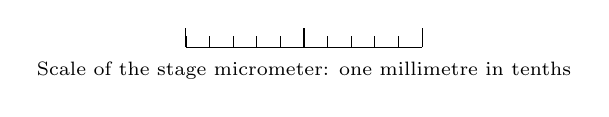
\begin{tikzpicture}[x=1cm,y=1cm]
  \draw[line width=.4pt] (0,0) -- (3,0);
  \foreach \x in {0,.3,...,3} { \draw[line width=.3pt] (\x,0) -- (\x,.14); }
  \foreach \x in {0,1.5,3} { \draw[line width=.4pt] (\x,0) -- (\x,.24); }
  \node[font=\scriptsize] at (1.5,-.3) {Scale of the stage micrometer:
    one millimetre in tenths};
\end{tikzpicture}
\end{center}

\vspace{.6em}
\footnotesize\noindent
Figures 2 to 4 are grown by rewriting grammars rather than drawn by hand. One
rule produces a single arm; six rotated copies supply the hexagonal symmetry
that a real crystal takes from its lattice, and a second set turned by thirty
degrees gives the twinned form. The hatched surround and clipped
circular field imitate the appearance of a plate engraved from the microscope
eyepiece, and the crystals stay vector paths at every magnification.

\end{document}
